\section{Testing da parte degli utenti}
In questa sezione, è riportato il protocollo di testing definito, una descrizione circa la sua esecuzione e la valutazione dei risultati raccolti
\subsection{Progettazione del test}
\label{subsubsection:progettazione-del-test}
Per testare le risorse esistenti, abbiamo ritenuto opportuno adottare l'approccio \textit{Discount Usability testing} (anche detto \textit{Guerrilla Usability Testing}), in quanto è maggiormente rispondente alle nostre esigenze: 
\begin{itemize}
    \item il presente progetto è di carattere didattico, per cui il budget a disposizione è molto limitato, il che si traduce nell'impossibilità di assumere assistenti, quali manager, psicologi e tecnici di vario genere per condurre il test;
    \item a causa della emergenza sanitaria in atto, minori sono le probabilità di riuscire a coinvolgere un numero elevato di soggetti da sottoporre al test;
\end{itemize}

\subsubsection{Task testati}
I task che abbiamo sottoposto agli utenti sono istanze dei task individuati nella fase ``Analisi dei task" e sono i seguenti:
\begin{itemize}
    \item calcolare il tasso di positività (calcolato come il rapporto tra nuovi positivi e i tamponi effettuati) relativo al 17 novembre;
    \item valutare l'occupazione dei reparti di terapia intensiva al 17 novembre
    \item calcolare il tasso di letalità (calcolato come il rapporto tra numero di deceduti e numero di casi) nel mese di Aprile
    \item calcolare il numero totale dei casi e il numero dei decessi per diverse fasce di età;
    \item confrontare l'andamento dei nuovi positivi giornalieri tra Emilia Romagna e Lombardia
    \item confrontare la media dei nuovi positivi giornalieri tra il mese di Aprile e il mese di Maggio;
\end{itemize}

\subsubsection{Tipologia di test}
Per quanto riguarda la tipologia di test, abbiamo adottato quella sommativa, in quanto la dashboard del DPC su cui realizzare i test è un applicazione web la cui fase di progettazione è stata già completata: conseguentemente, il fine del test è la ricerca di eventuali problemi che non sono stati scoperti e risolti dagli sviluppatori, nonché la verifica del soddisfacimento delle necessità raccolte all'inizio della progettazione.

\subsubsection{Ambito di test}
L'ambito del test è stato globale, dal momento che la dashboard del DPC fornisce a tutti i suoi utenti la possibilità di interagire con ogni sua funzione.

\subsubsection{Ambiente di test}
Il setting in cui verranno condotti i test ha visto l'utilizzo di software di videoconferenza. Gli assistenti del test siamo stati noi stessi, in qualità di membri del team di design. La selezione dei partecipanti è avvenuta mediante l'invio di una mail agli indirizzi dei giornalisti precedentemente contattati in occasione della ricerca etnografica.

\subsubsection{Dati raccolti}
I dati che sono stati raccolti hanno natura quantitativa: in dettaglio, abbiamo chiesto ad ogni giornalista di condurre certi task sull'interfaccia della dashboard del DPC e abbiamo preso nota del numero di problemi emersi, nonché una misura del loro impatto sull'esperienza dell'utente. L'output del test si è concretizzato, pertanto, in un insieme di valori numerici relativi ai giornalisti per ogni task, da cui abbiamo potuto calcolarci la frequenza di ogni problema.
Dato l'esiguo numero di giornalisti che si sono offerti per il test (7), non abbiamo potuto estrarre informazioni statisticamente significative, tuttavia abbiamo potuto raccogliere importanti suggerimenti di miglioramento circa l'usabilità dell'interfaccia.

\subsection{Selezione e preparazione degli assistenti}
Come riportato sopra, il test non ha previsto assistenti esterni, bensì è stato svolto interamente dai noi stessi, in qualità di membri del team di design. Abbiamo, a tal fine, studiato l'interfaccia della dashboard in oggetto, nonché applicato le nozioni apprese durante il corso di \textit{Usability \& User Experience Design}.

\subsection{Test pilota}
Il test pilota è stato condotto da noi stessi, in qualità di membri del team, tramite cui si è validato il protocollo definito in \ref{subsubsection:progettazione-del-test}: in dettaglio, si è verificata l'esistenza del c.d. happy path, il corretto funzionamento della piattaforma di videoconferenza scelta, il timing totale del test e l'appropriatezza delle richieste.

\subsection{Scelta dei partecipanti}
Per la scelta dei partecipanti, abbiamo cercato contatti di soggetti afferenti alla segmentazione dell'utenza elaborata nella sezione "Ricerca etnografica". Un criterio che abbiamo seguito è la diversificazione della redazione di riferimento (testata locale, nazionale, d'agenzia ecc.), al fine di avere risultati privi di bias.

\subsection{Esecuzione del test}
Il test è stato eseguito sulla dashboard del DPC (\href{https://opendatadpc.maps.arcgis.com/apps/opsdashboard/index.html#/b0c68bce2cce478eaac82fe38d4138b1}): trattasi di un'applicazione web totalmente funzionante.
\subsubsection{Approccio adottato}
L'approccio seguito è stato quello del \textit{"Thinking aloud"} per cui abbiamo chiesto a ciascun giornalista di eseguire task pre-determinati sull'interfaccia e di riferirci, appunto a voce alta, le sue impressioni e intenzioni step by step.

In questa maniera, abbiamo potuto registrare il numero di errori compiuto da ciascuno e una misura di gravità degli stessi: in dettaglio, i dati sono stati raccolti in una tabella.

\renewcommand{\arraystretch}{2}
\begin{longtable}{|c|p{7cm}|p{5cm}|c|}
    \hline
    \textbf{Nr} & \textbf{Problema} & \textbf{Frequenza (\%)} & \textbf{Impatto} \\
    \hline
    \endhead
    1 & Trovare il dato "tamponi effettuati" (l'utente è uscito dalla dashboard per prendersi il pdf del DPC): è possibile solo con molti step intermedi che richiedono il calcolo della differenza dei tamponi totali del giorno di interesse con quelli del giorno precedente, per ogni regione, e poi la somma fra queste differenze. & 80\% (Potrebbe capitare spesso visto che il dato proprio non esiste aggregato e deve essere computato manualmente) & Alto \\ \hline
    2 & L'utente dalla dashboard clicca su "Schede riepilogo PDF" come ultima spiaggia per trovare il dato "tamponi effettuati", ma non trova subito il pdf che cerca (quello giornaliero pubblicato dalle agenzie di stampa alle ore 17-18) & 10\% (Potenzialmente bassa, dipende se il giornalista già sa che là dentro troverà - forse - quello che cerca) & Basso \\ \hline
    3 & L'utente riesce a trovare le ospedalizzazioni attuali  + terapie intensive a granularità regionale, ma non nazionale (quindi andrebbero aggregate). Per quanto riguarda la disponibilità di posti nelle strutture ospedaliere non sono presenti dati nemmeno a livello regionale. & 70\% (Potrebbe capitare spesso visto che il dato proprio non esiste aggregato e deve essere computato manualmente) & Alto \\ \hline
    4 & L'utente vuole calcolare il tasso di letalità di un periodo predeterminato (deceduti/totale casi) ma ha avuto difficoltà a cercare i dati relativi a questo periodo (ha dovuto manualmente effettuare le sottrazioni raccogliendo prima i dati per la giornata di inizio e fine del periodo) dato che la dashboard non permette di selezionare range di date. & 20\% (bassa) & Medio \\ \hline
    5 & I dati per età non sono disponibili direttamente nella dashboard. L'utente può trovarli seguendo alcuni link a un file Excel nella pagina in cui si trova la dashboard dell'ISS ("concorrenza"). & 20\% (bassa) & Alto \\ \hline
    6 & L'utente può recuperare il dato dei nuovi positivi nazionali e regionali, ma manca un etichetta chiara (questo dato è chiamato "Incremento" quando ci si riferisce al totale dei casi riscontrati dall'inizio della pandemia) & 100\% & Basso \\ \hline
    7 & L'utente vuole calcolare l'incremento di nuovi positivi di un periodo predeterminato, ma ha avuto difficoltà a raccogliere i dati relativi a questo periodo (ha dovuto manualmente effettuare le sottrazioni raccogliendo prima i dati per la giornata di inizio e fine del periodo) dato che la dashboard non permette di selezionare range di date. & 20\% & Basso \\ \hline
\end{longtable}

\subsection{Valutazione finale e report}
Abbiamo valutato i dati raccolti calcolando la frequenza degli errori dei diversi giornalisti a fronte di ciascun task e tracciando una curva di urgenza (\ref{fig:urgency-curves}) in termini di frequenza e impatto dei problemi emersi.
Dal grafico  si evince che i problemi maggiori e quindi più urgenti da risolvere sono 1, 3, 5 e 6. Il problema nr. 5 ha un impatto molto alto anche se è poco frequente e  6 in quanto anche se è poco impattante è molto frequente.

\begin{figure}[H]
    \centering
    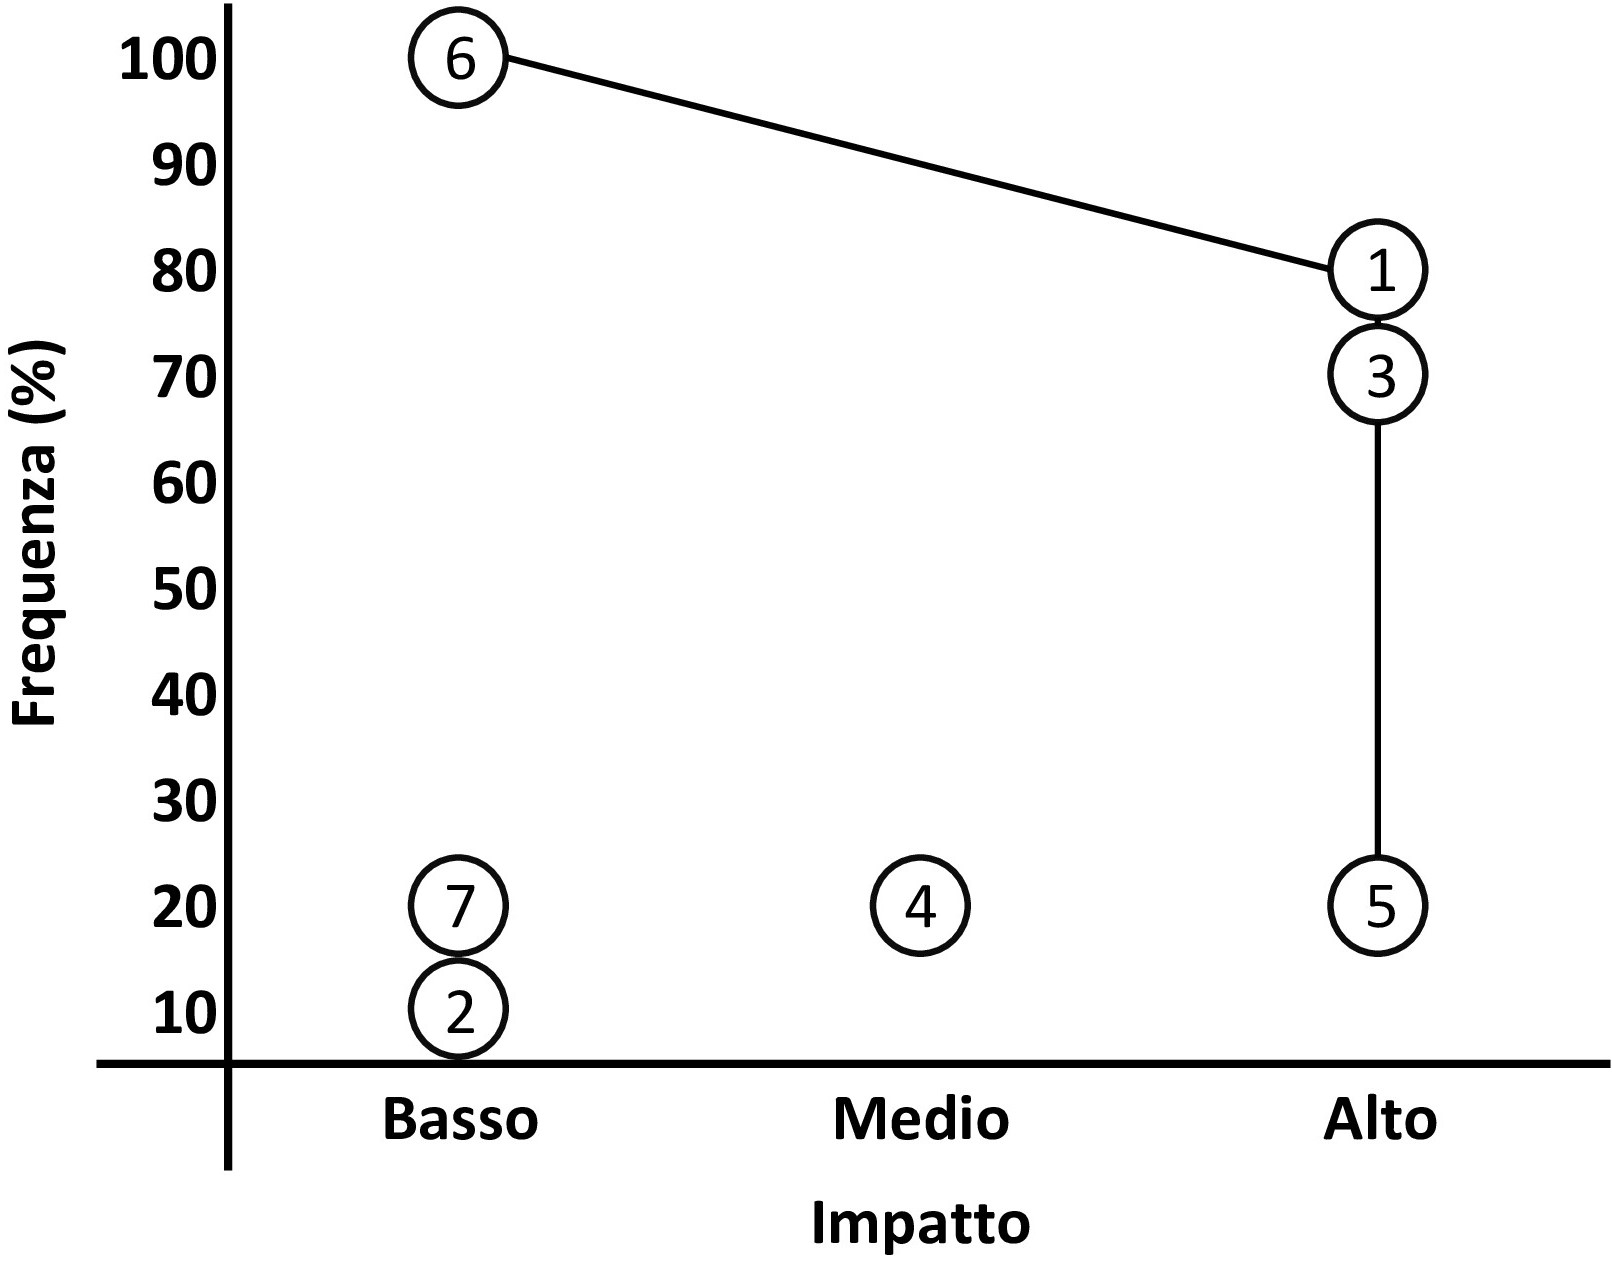
\includegraphics[width=0.5\columnwidth]{../../../assets/images/verifica-risorse-esistenti/urgency_curve}
    \caption{Curva delle urgenze.}
    \label{fig:urgency-curves}
\end{figure}
